\def\QRCODE{TB_image_TUT.IMG.image_restoration_deblurring_pythonqrcode.png}
\def\QRPAGE{http://www.iptutorials.science/tree/master/TB_image/TUT.IMG.image_restoration_deblurring/python}
\pcorrectionsection{Python correction}

\begin{python}
from astropy.io import fits
import matplotlib.pyplot as plt
import numpy as np
from scipy.misc import imresize
from scipy import signal
import progressbar
\end{python}

\vspace*{-3pt}

\subsection{Damage modeling}

\textls[-25]{There is no built-in function to generate the checkerboard image. A simple code can be used.}
\begin{python}
def checkerboard():
    arr = np.zeros((8,8),dtype=int)
    arr[::2,::2] = 1
    arr[1::2,1::2] = 1
    out = imresize(arr,8*np.array(arr.shape),interp='nearest')/255;
    return out;
\end{python}

The psf can be generated as a Gaussian psf, or a motion psf. In this tutorial, the motion psf is loaded from a file that comes from the \matlabregistered{} function \minline{fspecial}.%%pbsparta
\begin{python}
C = checkerboard();
psf = np.load('psf_motion.npy');
\end{python}

In order to add Gaussian noise, the following function is used:
\begin{python}    
def addGaussianNoise(I, sigma=1000):
    """Adds Gaussian noise to an image
    I: original image
    sigma: signal/noise ratio
    """
    I2 = I.copy();
    m=np.min(I);
    M=np.max(I);
    N = (M-m)/sigma*np.random.randn(I.shape[0], I.shape[1]);
    I2 = I2 + N;
    I2[I2>M] = M;
    I2[I2<m]=m;
    return I2, I-I2;
\end{python}

The image is blurred and noise is then added.
\begin{python}
Cb = signal.convolve2d(C, psf, boundary='wrap', mode='same');
Cbn, noise = addGaussianNoise(Cb);
plt.imshow(Cbn, cmap='gray')
plt.title('Motion blur + Gaussian noise on checkerboard')
plt.show();
\end{python}

\subsubsection{Optical Transfer Function: OTF}
The OTF is the centered Fourier Transform of the PSF (Point Spread Function). The following function is used to get the OTF from the PSF:
\begin{python}
def psf2otf(psf, s):
    """
    Get OTF (Optical Transfer Function) from PSF (Point Spread Function)
    OTF is basically the Fourier Transform of the PSF, centered
    psf: PSF 
    s: shape of the result, zero-padding is used to center is Fourier Transform
    """
    sh = psf.shape;
    sh = np.array(sh);
    s = np.array(s);
    pad = s - sh;
    h = np.pad(psf, ((0,pad[0]), (0, pad[1])), mode='constant');
    shift = (int(pad[0]/2+1), int(pad[1]/2+1));
    h_centered = np.roll(h, tuple(shift), axis=(0,1));
    h_centered = np.fft.fftshift(h_centered);
    H = np.fft.fft2(h_centered, s);
    H = np.real(H);
    return H;
\end{python}

\vspace*{-8pt}

\subsection{Simple case: no noise}
For the direct reconstruction, just ensure that there is no division by 0. The different results are illustrated in Fig.\ref{fig:deblurring:python:checkerboard}.

\begin{python}
H = psf2otf(psf, C.shape);
G = np.fft.fft2(Cb);
alpha =  0.001;
F = G / (H+alpha);
fr = np.real(np.fft.ifft2(F));
plt.imshow(fr);
plt.title('Noiseless (only motion blur) direct reconstruction')
plt.imsave("cb_reconstruction.png", fr, cmap='gray');
plt.show()
\end{python}

In the presence of noise, the reconstructed image is not perfect.
\begin{python}
H = psf2otf(psf, C.shape);
G = np.fft.fft2(Cbn);
alpha =  0.001;
F = G / (H+alpha);
fr = np.real(np.fft.ifft2(F));
\end{python}

The automatic evaluation of the noise parameter is done in the Wiener filter by:
\begin{python}
SpecPuissNoise=np.abs(np.fft.fft2(noise))**2;
PuissMoyNoise=np.mean(SpecPuissNoise);
SpecPuissImageOrig=np.abs(np.fft.fft2(C))**2;
PuissMoyImageOrig=np.mean(SpecPuissImageOrig);
ratio=PuissMoyNoise/PuissMoyImageOrig;
Hw = np.conjugate(H)/(np.abs(H)**2+ratio);
fr = np.fft.ifft2( Hw * np.fft.fft2(Cbn));
\end{python}

\subsection{Iterative filters}
\subsubsection{Van-Cittert iterative filter}
The parameter (Jansson parameter) controls the precision of convergence, but a small value requires a high number of iterations (and thus a high computation time).
\begin{python}
def vca(g, psf, n_iter, beta=.01):
    """
    Van Cittert iterative filter
    g: noisy image
    psf: point spread function
    n_iter: number of iterations
    beta: Jansson parameter
    """
    H = psf2otf(psf, g.shape);
    
    # init iterations
    fr = g.copy();
    bar = progressbar.ProgressBar();
    for iter in bar(range(n_iter)):
        estimation = np.real(np.fft.ifft2(H * np.fft.fft2(fr)));
        fr= fr + beta* ( g - estimation);
        
    return fr; 
\end{python}

\subsubsection{Richardson-Lucy iterative filter}
This algorithm is probably the most famous one in the domain. Remember that the symmetry in the space domain becomes the complex conjugate in the spectral domaine (after Fourier transform).
\begin{python}
def rla(g, psf, n_iter):
    """
    Richardson Lucy algorithm
    g: noisy image
    psf: point spread function
    n_iter: number of iterations
    """
    H = psf2otf(psf, g.shape); 
    # init iterations
    fr = g.copy();
    
    bar = progressbar.ProgressBar()
    for iter in bar(range(n_iter)):
        estimation = np.fft.ifft2(H * np.fft.fft2(fr));
        M = np.real(np.fft.ifft2(np.conjugate(H) * np.fft.fft2(g / estimation)));
        fr= fr * M;
        fr[fr<0] = 0;
        
    return fr;
\end{python}


\begin{figure}[H]
\centering\caption{Different deconvolution methods applied on the synthetic image 'checkerboard'.}%
\subfloat[Damaged checkerboard image, with motion blur and Gaussian noise.]{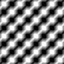
\includegraphics[width=.3\linewidth]{cbn_original.png}}
\hfill
\subfloat[Reconstruction of the che\-cker\-board without noise.]{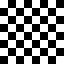
\includegraphics[width=.3\linewidth]{cb_reconstruction.png}}
\hfill
\subfloat[Reconstruction of the che\-cker\-board with noise.]{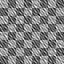
\includegraphics[width=.3\linewidth]{cbn_reconstruction.png}}

\subfloat[Wiener deconvolution.]{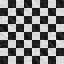
\includegraphics[width=.3\linewidth]{cbn_wiener.png}}
\hfill
\subfloat[Van-Cittert iterative deconvolution with 100 iterations, and Jansson parameter at 0.01.]{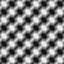
\includegraphics[width=.3\linewidth]{cbn_vca.png}}
\hfill
\subfloat[Richardon-Lucy iterative de\-con\-vo\-lu\-tion with 1000 iterations.]{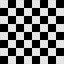
\includegraphics[width=.3\linewidth]{cbn_rla.png}}

\subfloat[Landweber iterative de\-con\-vo\-lu\-tion with 1000 iterations and Jansson parameter at 1.]{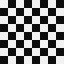
\includegraphics[width=.3\linewidth]{cbn_lva.png}}
\hfill
\subfloat[Poisson Maximum A Posteriori iterative deconvolution with 1000 iterations.]{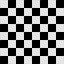
\includegraphics[width=.3\linewidth]{cbn_pmap.png}}%
\label{fig:deblurring:python:checkerboard}
\end{figure}

\newpage

\subsection{Astronomy images}
These real images come from the Hubble Space Telescope (HST, see credits), shown in Fig.\ref{fig:deblurring:python:astronomy}. The results for the Richardson-Lucy, Van-Cittert and Landweber algorithms are shown in Fig.\ref{fig:deblurring:python:astro_reconstruction}. The direct deconvolution does not give a correct result.

\begin{figure}[htbp]
\centering\caption{Original images and PSF, from the HST.}
\subfloat[Jupiter.]{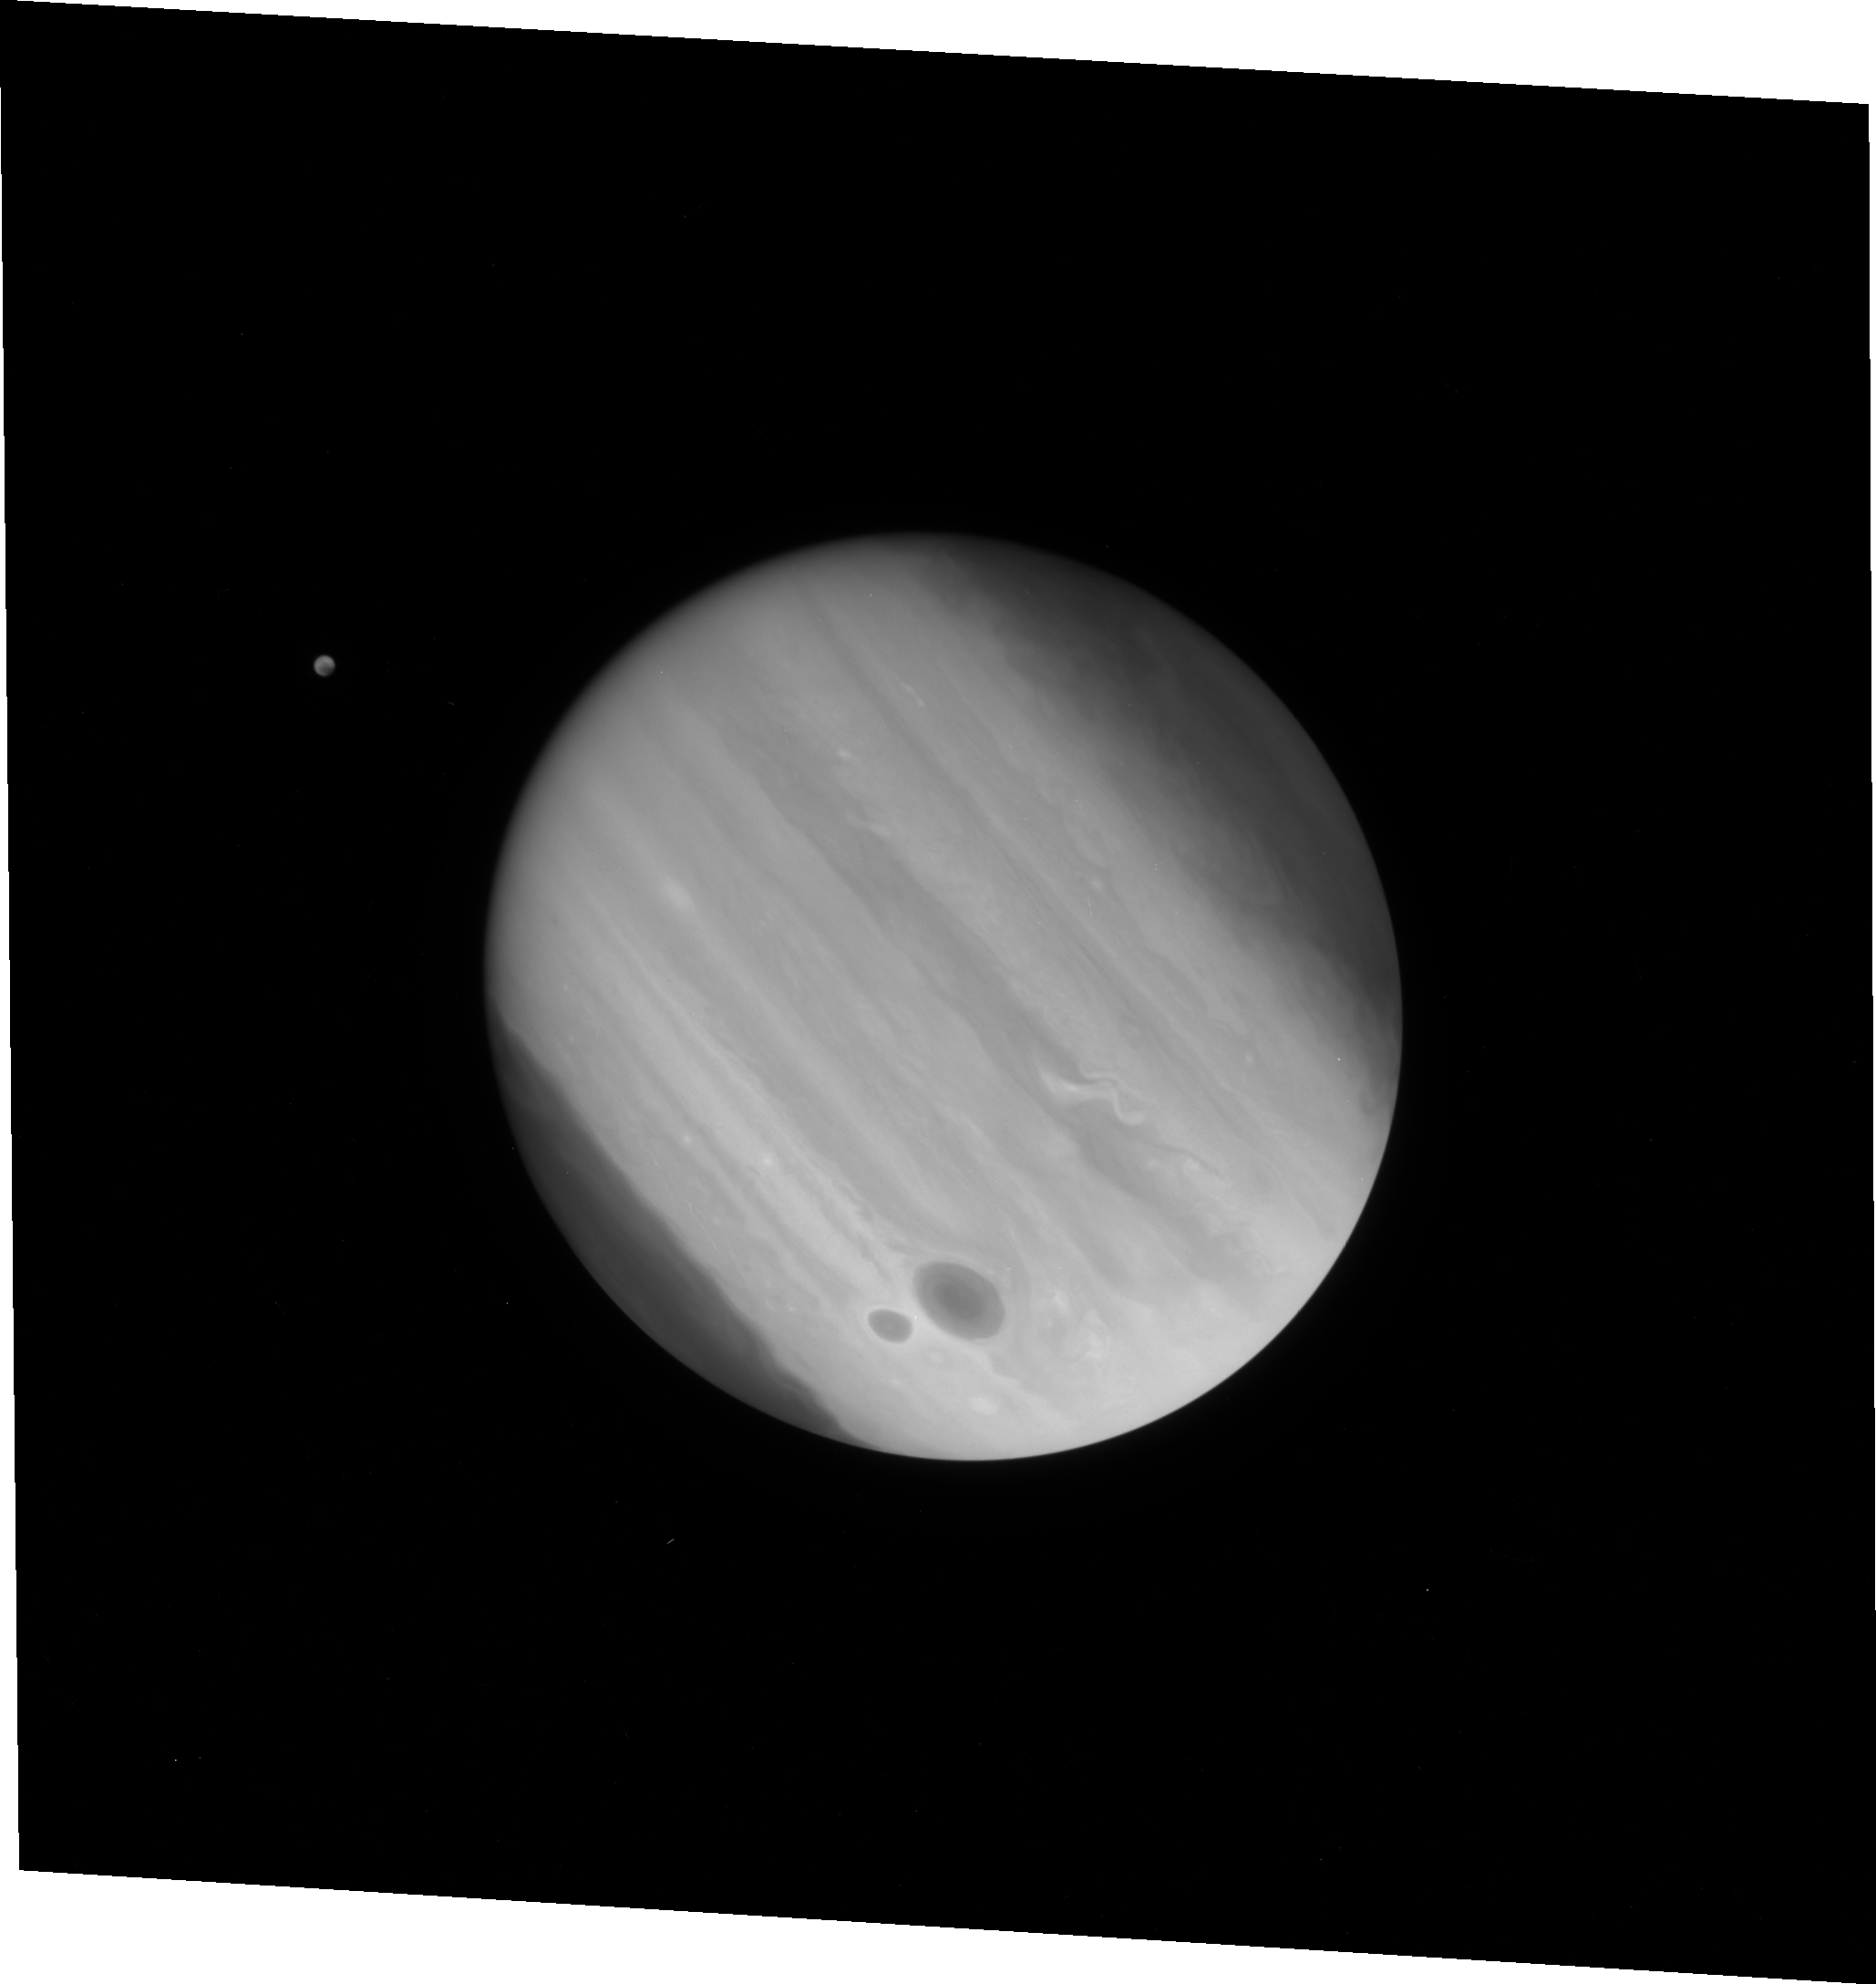
\includegraphics[width=.45\linewidth]{jupiter.png}}\hfill
\subfloat[PSF for the observation of Jupiter.]{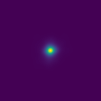
\includegraphics[width=.45\linewidth]{jupiter_psf.png}}

\subfloat[Saturn.]{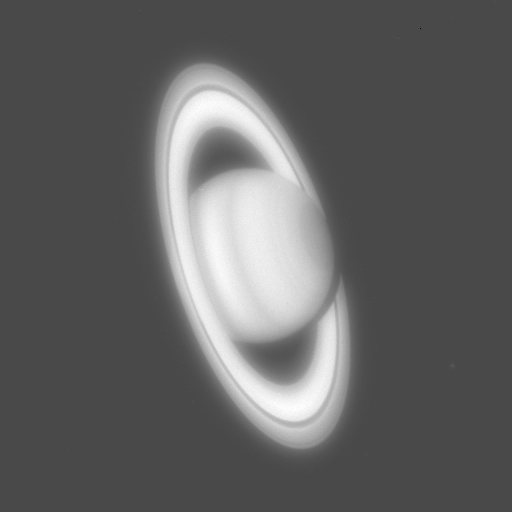
\includegraphics[width=.45\linewidth]{saturn.png}}\hfill
\subfloat[PSF for the observation of Saturn.]{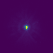
\includegraphics[width=.45\linewidth]{saturn_psf.png}}%
\label{fig:deblurring:python:astronomy}%
\end{figure}


\begin{figure}[htbp]
\caption{Different deconvolution methods applied for the astronomy images.}%
\subfloat[Direct deconvolution.]{
\includegraphics[width=.3\linewidth]{jupiter_direct.png}}
\hfill
\subfloat[Direct deconvolution.]{
\includegraphics[width=.3\linewidth]{saturn_direct.png}}

\subfloat[Richardon-Lucy iterative de\-con\-vo\-lu\-tion with 10 iterations.]{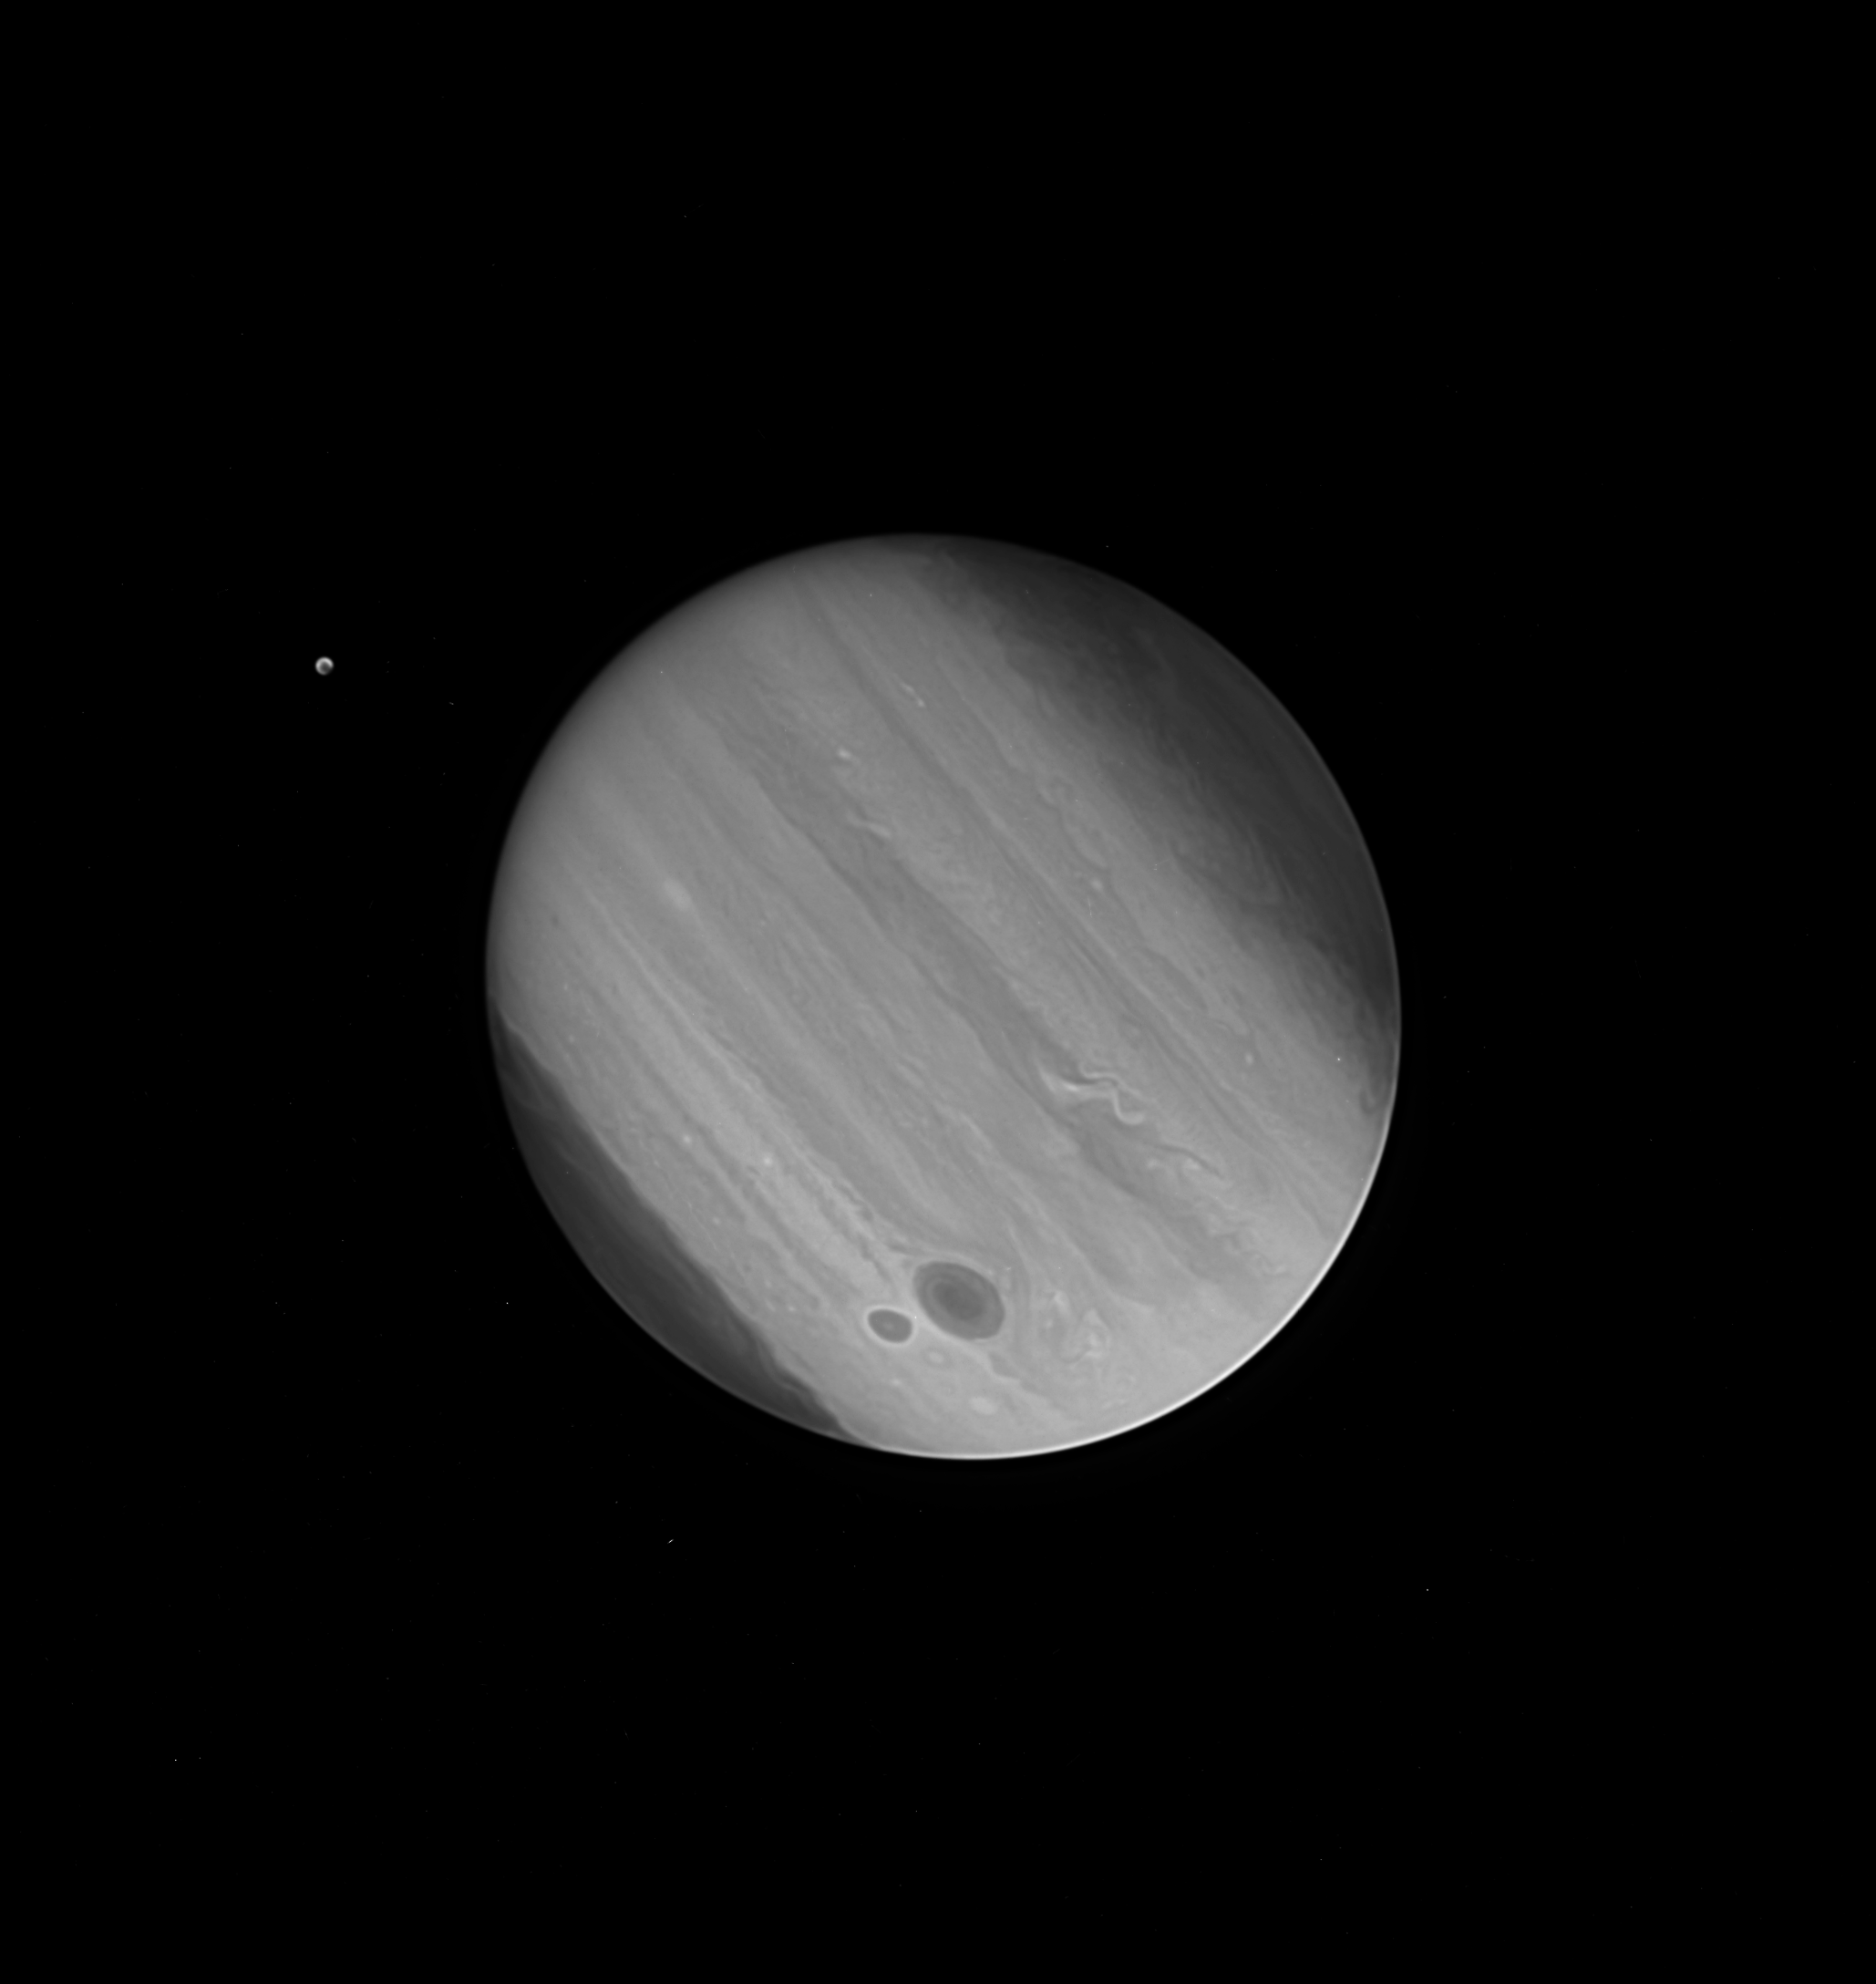
\includegraphics[width=.3\linewidth]{jupiter_rla.png}}
\hfill
\subfloat[Van-Cittert iterative de\-con\-vo\-lu\-tion with 10 iterations.]{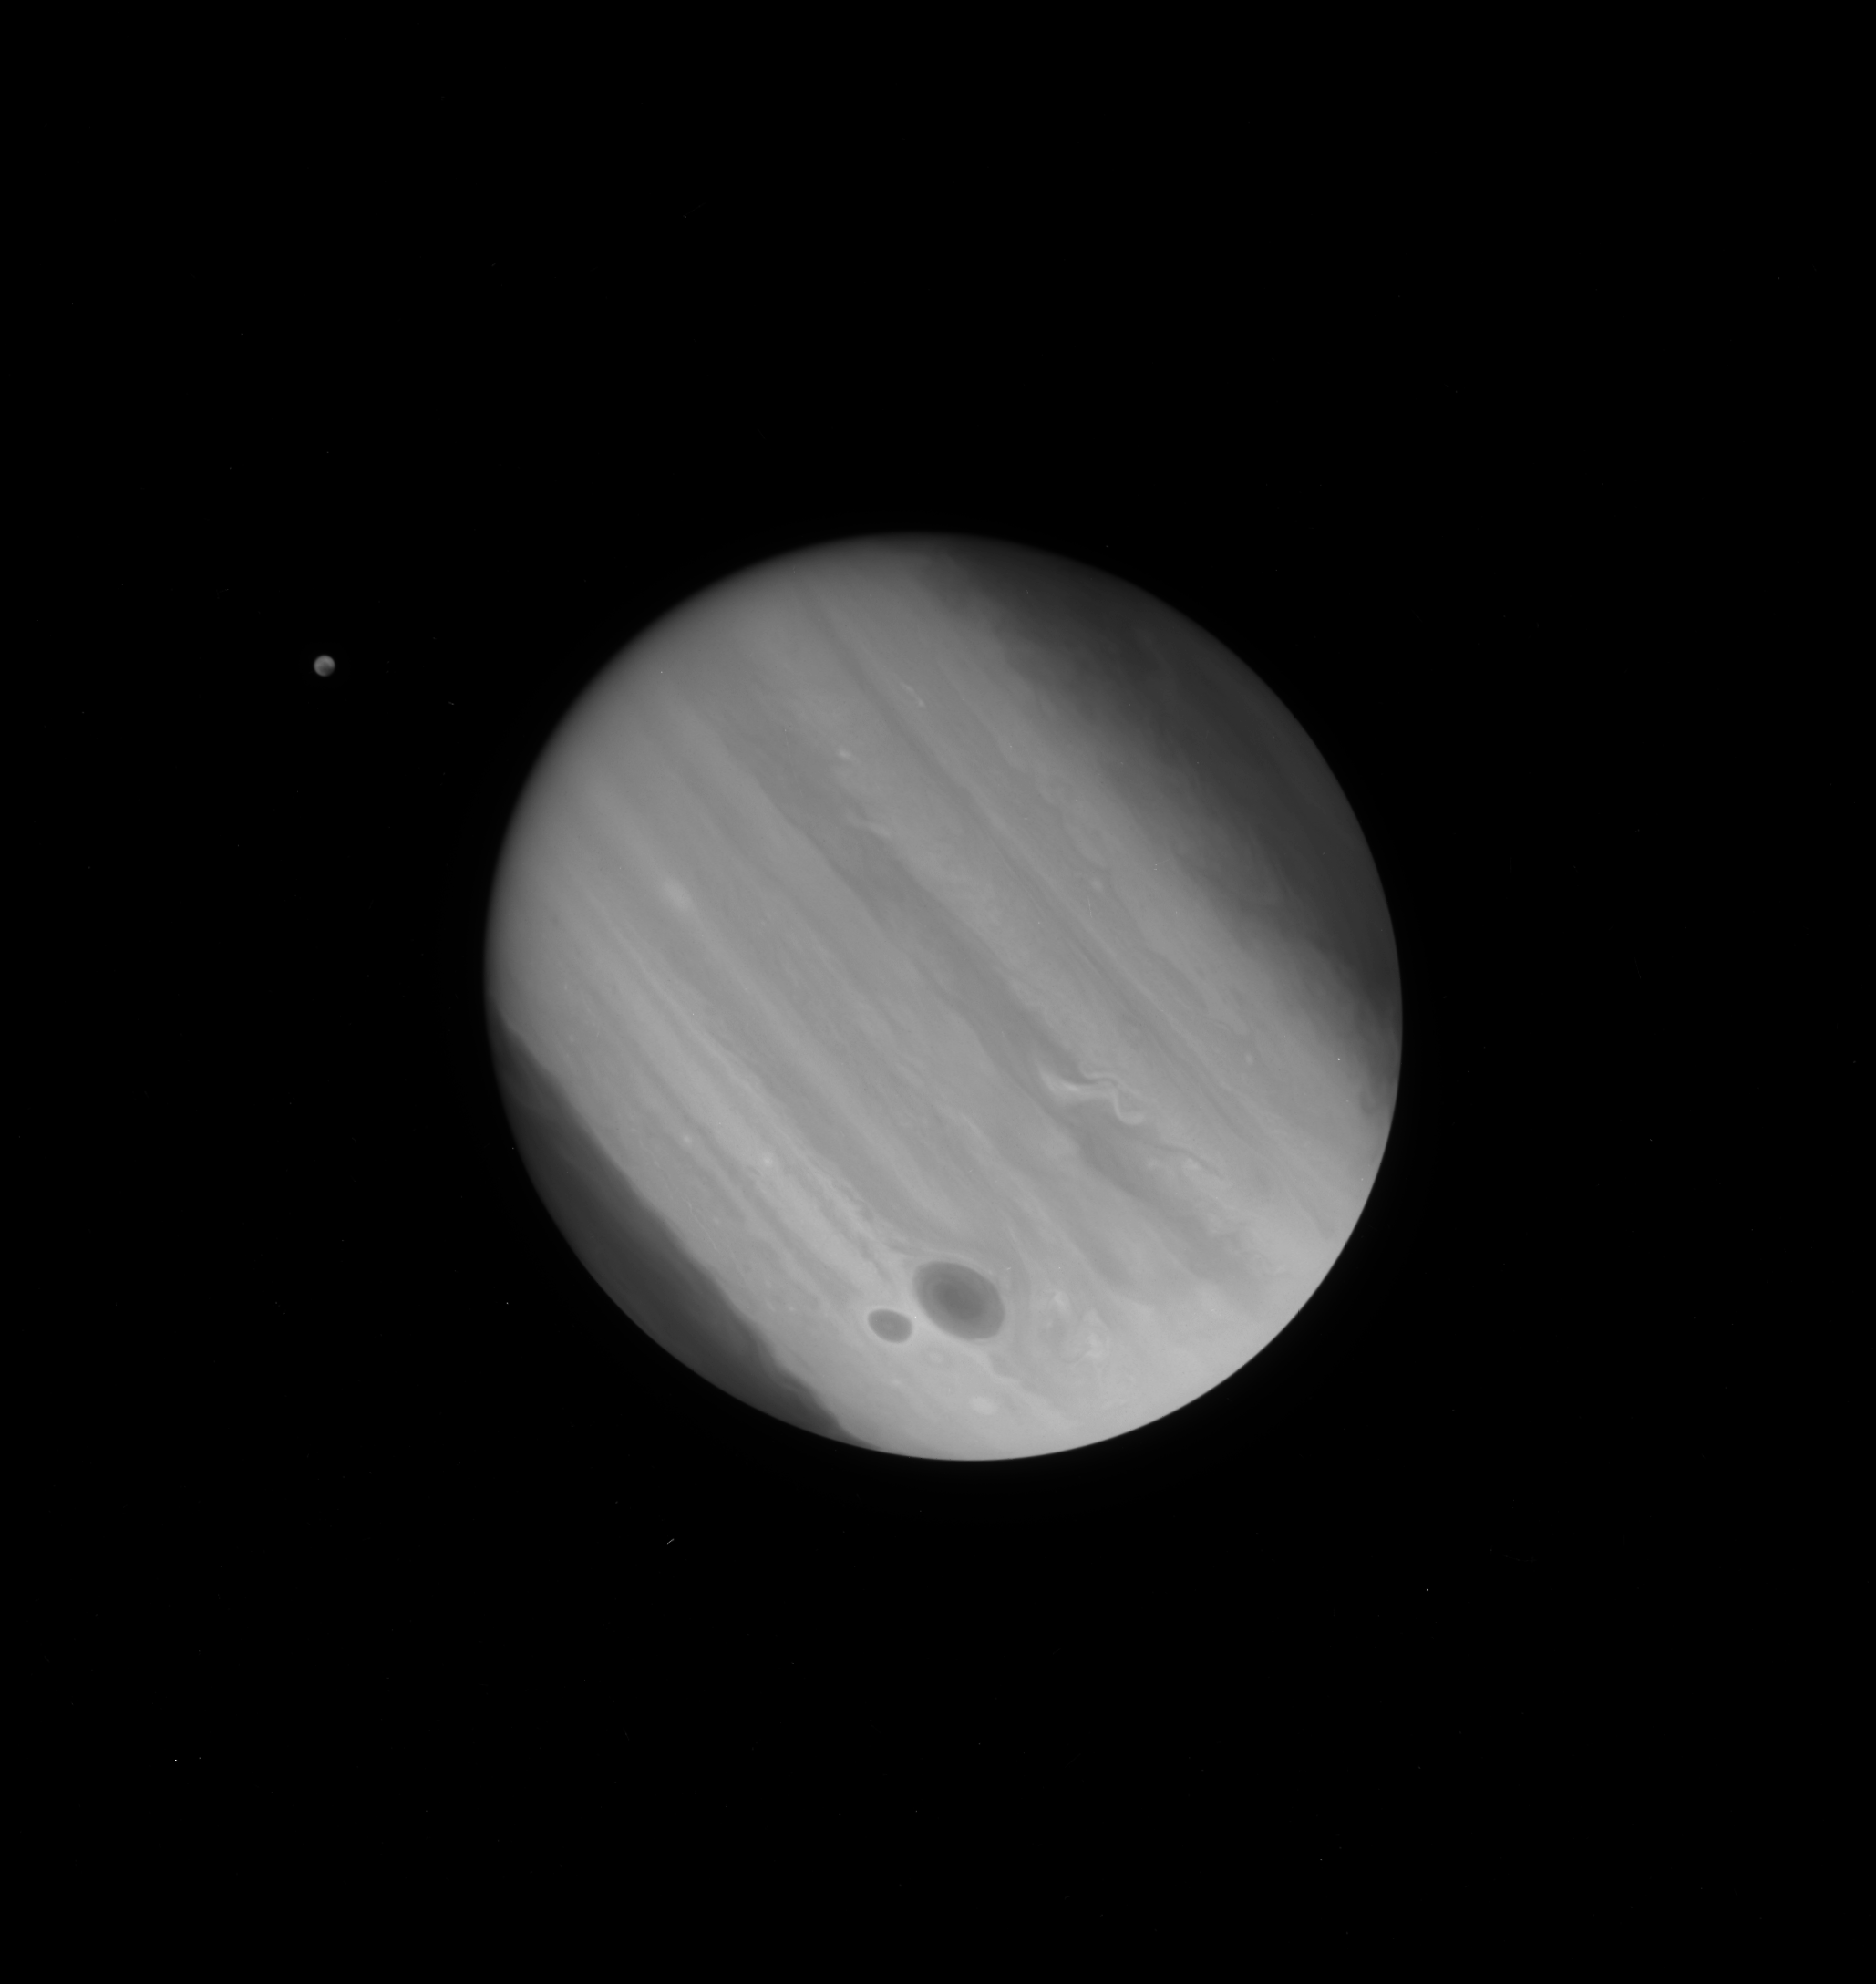
\includegraphics[width=.3\linewidth]{jupiter_vca.png}}
\hfill
\subfloat[Landweber iterative de\-con\-vo\-lu\-tion with 200 iterations and Jansson parameter at 1.]{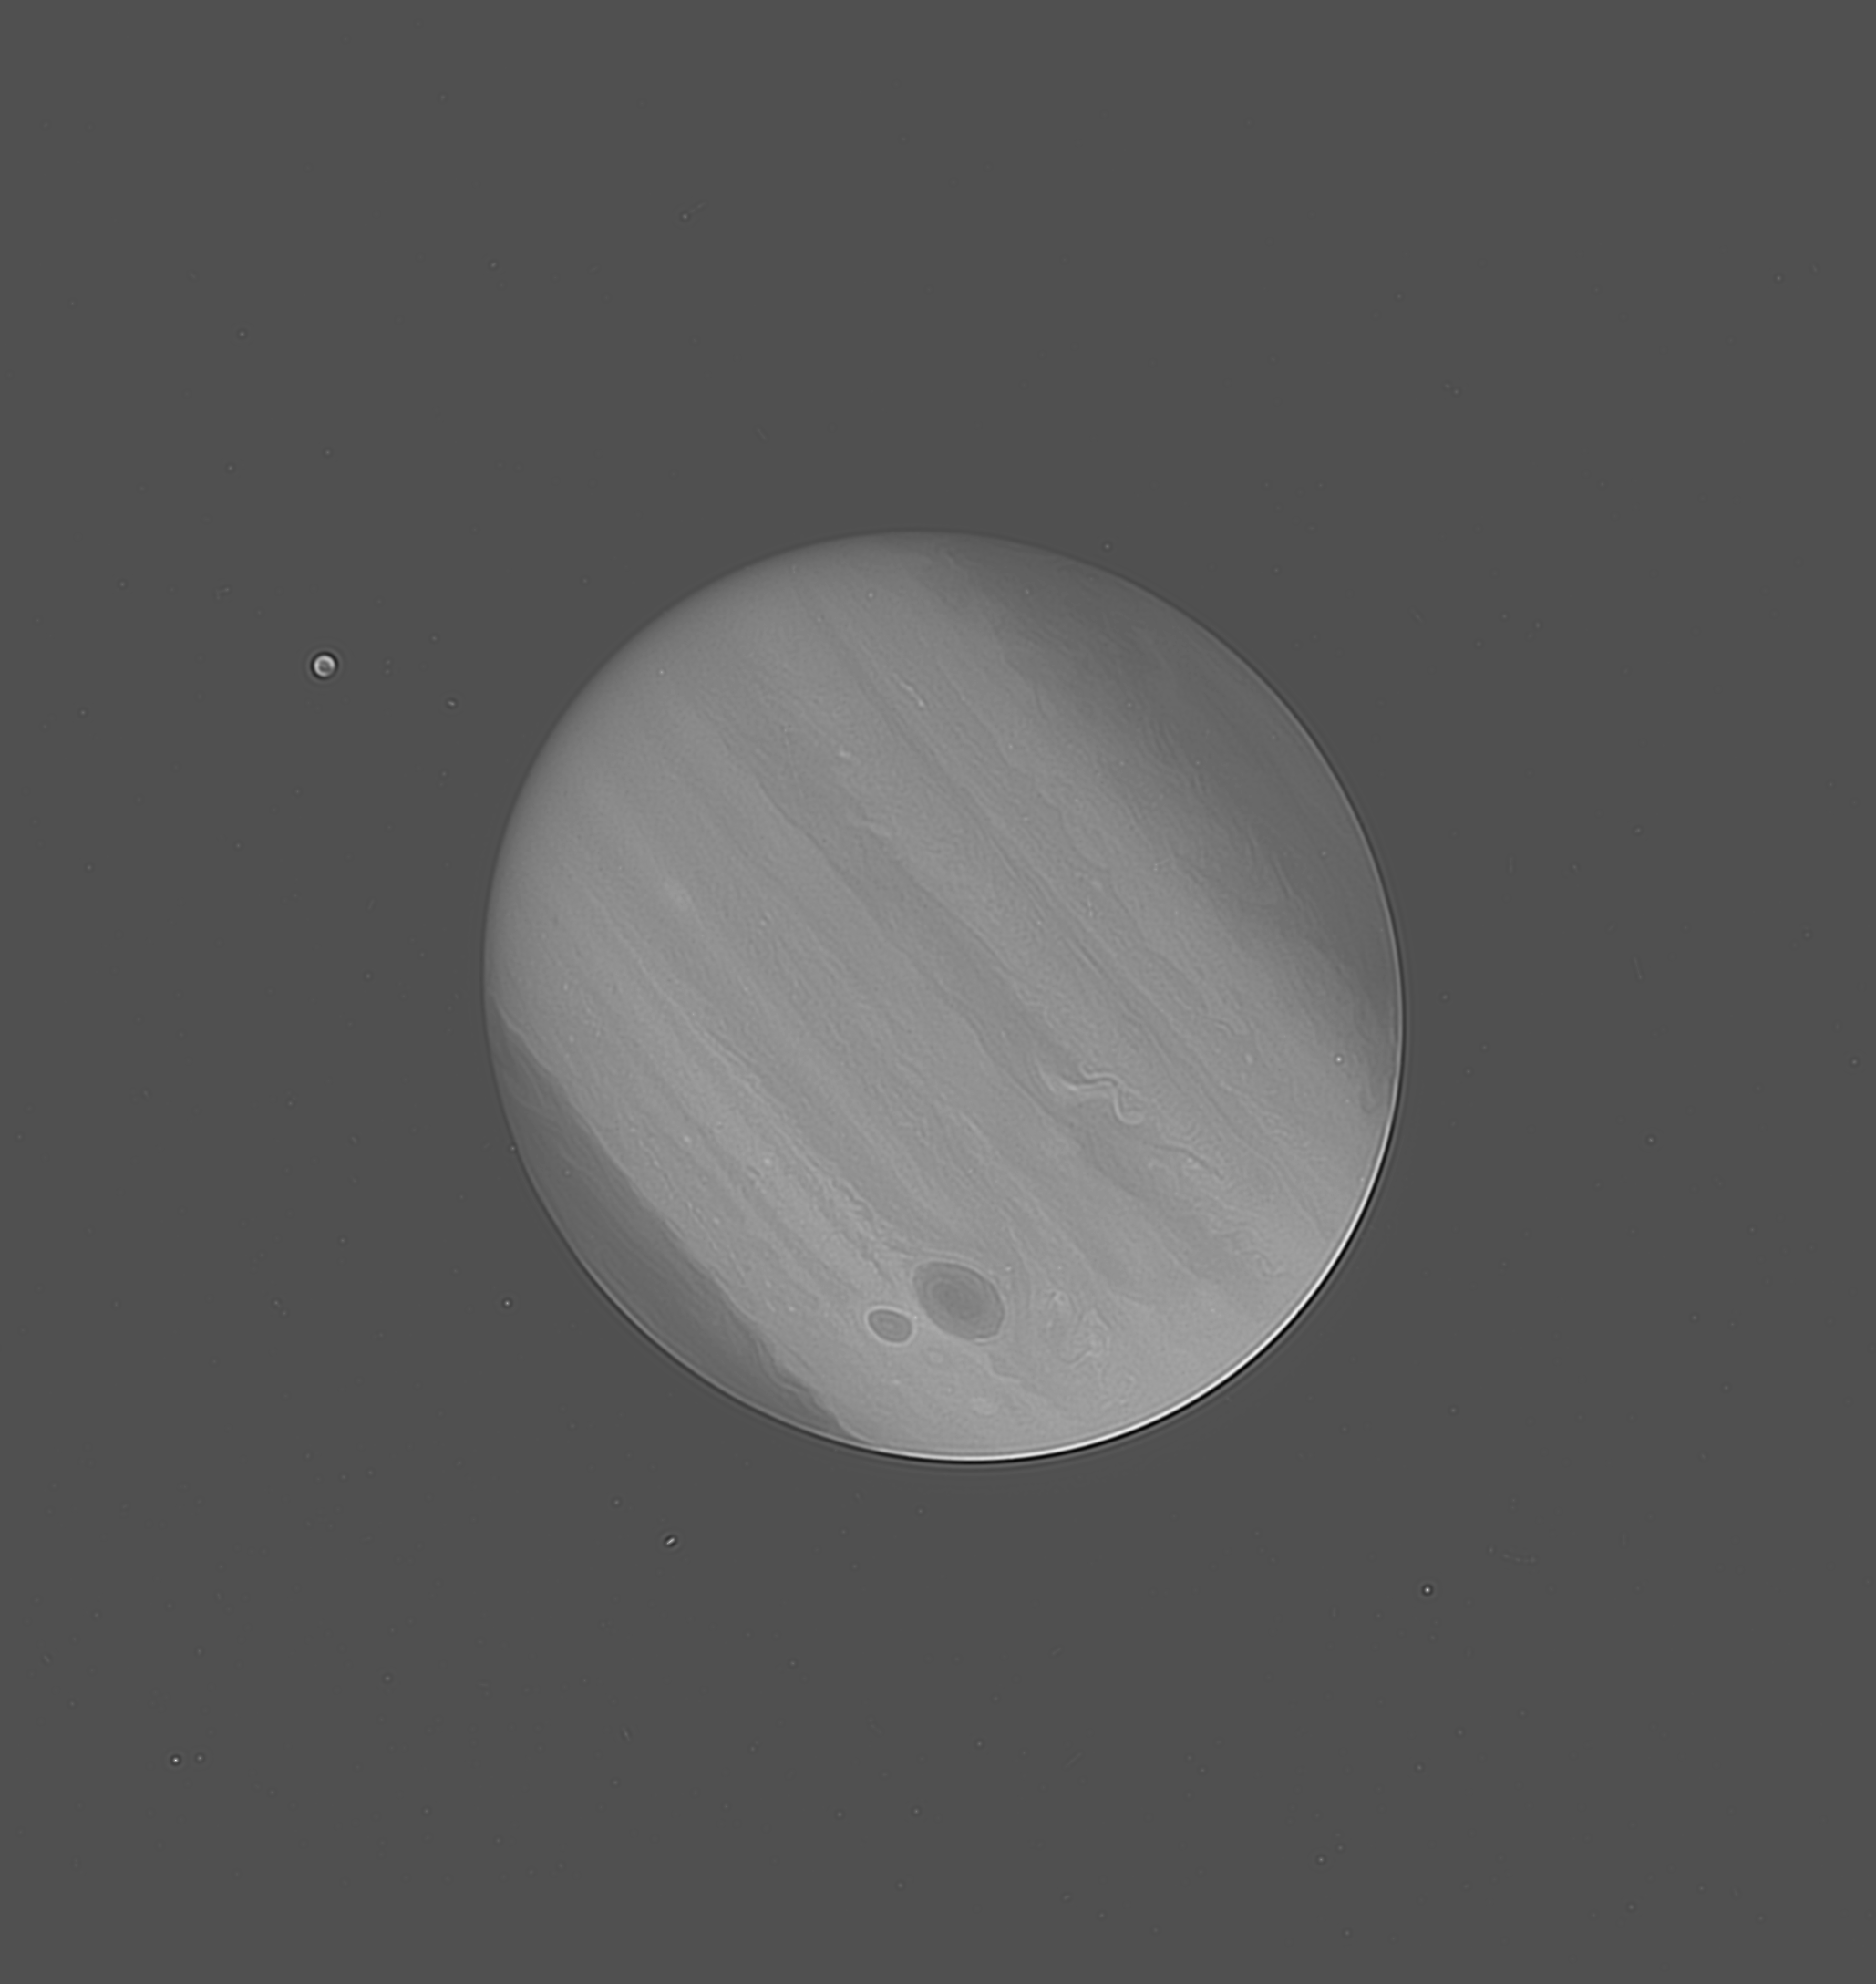
\includegraphics[width=.3\linewidth]{jupiter_lva.png}}

\subfloat[Richardon-Lucy iterative de\-con\-vo\-lu\-tion  with 10 iterations.]{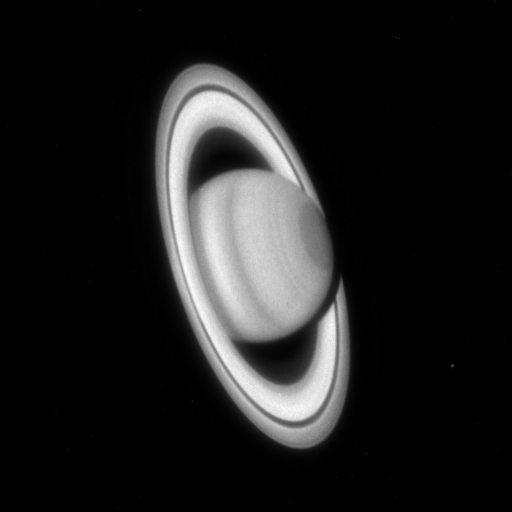
\includegraphics[width=.3\linewidth]{saturn_rla.png}}
\hfill
\subfloat[Van-Cittert iterative de\-con\-vo\-lu\-tion  with 10 iterations.]{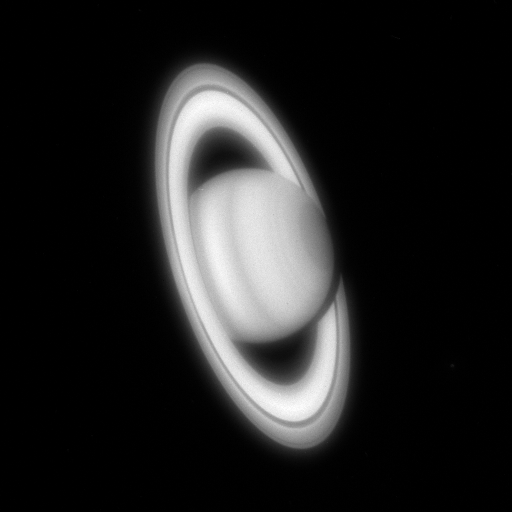
\includegraphics[width=.3\linewidth]{saturn_vca.png}}
\hfill
\subfloat[Landweber iterative de\-con\-vo\-lu\-tion  with 200 iterations and Jansson parameter at 1.]{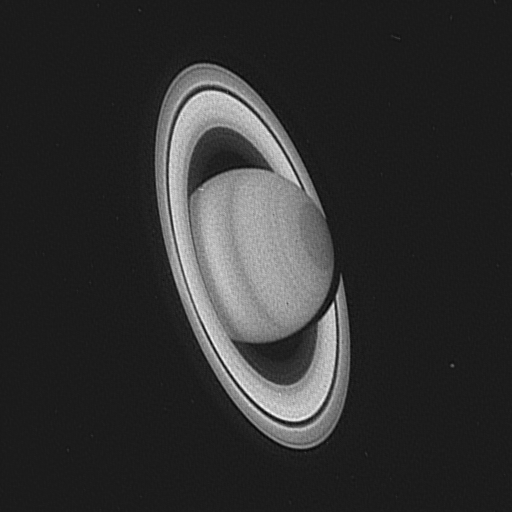
\includegraphics[width=.3\linewidth]{saturn_lva.png}}%
\label{fig:deblurring:python:astro_reconstruction}%
\end{figure}
